\begin{questions}


\question Write out all functions $f: \{1,2,3\}$ to $\{a,b\}$.  How many are there?  How many are injective?  How many are surjective?  How many are both?

	\begin{answer}
	There are 8 different functions.  For example, $f(1) = a$, $f(2) = a$, $f(3) = a$; or $f(1) = a$, $f(2) = b$, $f(3) = a$, and so on.  None of the functions are injective.  Exactly 6 of the functions are surjective.  No functions are both (since no functions here are injective).
	\end{answer}
	
	
	

\question Write out all functions $f: \{1,2\}$ to $\{a,b,c\}$.  How many are there?  How many are injective?  How many are surjective?  How many are both?

	\begin{answer}
	There are nine functions - you have a choice of three outputs for $f(1)$, and for each, you have three choices for the output $f(2)$.  Of these functions, 6 are injective, 0 are surjective, and 0 are both.
	\end{answer}
	
	
	

\question Consider the function $f:\{1,2,3,4,5\} \to \{1,2,3,4\}$ given by the table below:

\begin{center}
\begin{tabular}{c||c|c|c|c|c}
              $x$ & 1 & 2 & 3 & 4 & 5 \\ \hline
              $f(x)$ & 3 & 2 & 4 & 1 & 2
            \end{tabular}
\end{center}

\begin{parts}
  \part Is $f$ injective?  Explain.
  \part Is $f$ surjective?  Explain.
\end{parts}

	\begin{answer}
		\begin{parts}
		%Is $f$ injective?  Explain.
		\part $f$ is not injective, since $f(2) = f(5)$ - two different inputs have the same output. 
		% Is $f$ surjective?  Explain.
		\part $f$ is surjective, since every element of the codomain is an element of the range.
		\end{parts}
	\end{answer}
	
	
	

\question Consider the function $f:\{1,2,3,4\} \to \{1,2,3,4\}$ given by the graph below.
\begin{multicols}{2}
\begin{center}
  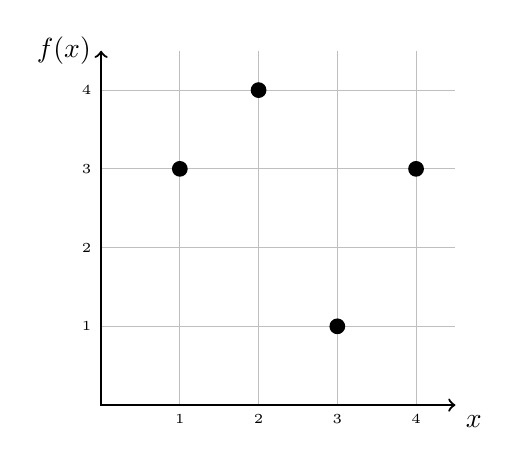
\begin{tikzpicture}[scale=1]
    \draw[thin, gray!50] (0,0) grid (4.5, 4.5);
    \draw[<->, thick] (0,4.5) node[left] {$f(x)$} -- (0,0) -- (4.5,0) node[below right] {$x$};
    \foreach \x in {1,2,3,4}
      \draw (\x,0) node[below] {\tiny \x} (0, \x) node[left] {\tiny \x};
    \fill (1,3) circle (.1) (2,4) circle (.1) (3,1) circle (.1) (4,3) circle (.1);
  \end{tikzpicture}
\end{center}

\begin{parts}
  \part Is $f$ injective?  Explain.
  \part Is $f$ surjective?  Explain.
\end{parts}
\end{multicols}


	\begin{answer}
		\begin{parts}
		%Is $f$ injective?  Explain.
		  \part $f$ is not injective, since $f(1) = 3$ and $f(4) = 3$.
		%   Is $f$ surjective?  Explain.
		  \part $f$ is not surjective, since there is no input which gives 2 as an output.
		\end{parts}
	\end{answer}
	
	
	


\question For each function given below, determine whether or not the function is injective and whether or not the function is surjective.
\begin{parts}
  \part $f:\N \to \N$ given by $f(n) = n+4$.
  \part $f:\Z \to \Z$ given by $f(n) = n+4$.
  \part $f:\Z \to \Z$ given by $f(n) = 5n - 8$.
  \part $f:\Z \to \Z$ given by $f(n) = \begin{cases}
                                         n/2 & \mbox{ if $n$ is even}\\
                                         (n+1)/2 & \mbox{ if $n$ is odd}.
                                       \end{cases}$
\end{parts}

	\begin{answer}
		\begin{parts}
		% $f:\N \to \N$ given by $f(n) = n+4$.
		  \part $f$ is injective, but not surjective.
		%   $f:\Z \to \Z$ given by $f(n) = n+4$.
		  \part $f$ is injective and surjective.
		  %$f:\Z \to \Z$ given by $f(n) = 5n - 8$.
		  \part $f$ is injective, but not surjective.
		%   $f:\Z \to \Z$ given by $f(n) = \begin{cases}
		%                                          n/2 & \mbox{ if $n$ is even}\\
		%                                          (n+1)/2 & \mbox{ if $n$ is odd}.
		%                                        \end{cases}$
		 \part $f$ is not injective, but is surjective.
		\end{parts}
	\end{answer}
	
	
	

\question Let $A = \{1,2,3,\ldots,10\}$.  Consider the function $f:\pow(A) \to \N$ given by $f(B) = |B|$.  So $f$ takes a subset of $A$ as an input and outputs the cardinality of that set.  
\begin{parts}
  \part Is $f$ injective?  Prove your answer.
  \part Is $f$ surjective?  Prove your answer.
  \part Find $f\inv(1)$.
  \part Find $f\inv(0)$.
  \part Find $f\inv(12)$.
\end{parts}

	\begin{answer}
		\begin{parts}
		% Is $f$ injective?  Prove your answer.
		  \part $f$ is not injective.  To prove this, we must simply find two different elements of the domain which map to the same element of the codomain.  Since $f(\{1\}) = 1$ and $f(\{2\}) = 1$, we see that $f$ is not injective.
		%   Is $f$ surjective?  Prove your answer.
		  \part $f$ is not surjective.  The largest subset of $A$ is $A$ itself, and $|A| = 10$.  So no natural number greater than 10 will ever be an output.
		%   Find $f\inv(1)$.
		  \part $f\inv(1) = \{\{1\}, \{2\}, \{3\}, \ldots \{10\}\}$ (the set of all the singleton subsets of $A$).
		%   Find $f\inv(0)$.
		  \part $f\inv(0) = \{\emptyset\}$.  Note, it would be wrong to write $f\inv(0) = \emptyset$ - that would claim that there is no input which has 0 as an output.
		   % Find $f\inv(12)$.
		  \part $f\inv(12) = \emptyset$, since there are no subsets of $A$ with cardinality 12.
		\end{parts}
	\end{answer}
	
	
	

\question Let $A = \{n \in \N \st 0 \le n \le 999\}$ be the set of all numbers with three or fewer digits.  Define the function $f:A \to \N$ by $f(abc) = a+b+c$, where $a$, $b$, and $c$ are the digits of the number in $A$.  For example, $f(253) = 2 + 5 + 3 =  10$.
\begin{parts}
  \part Find $f\inv(3)$.
  \part Find $f\inv(28)$.
  \part Use one of the parts above to prove that $f$ is not injective.
  \part Use one of the parts above to prove that $f$ is not surjective.
\end{parts}

	\begin{answer}
		\begin{parts}
		% Find $f\inv(3)$.
		  \part $f\inv(3) = \{003, 030, 300, 012, 021, 102, 201, 120, 210, 111\}$
		%   Find $f\inv(28)$.
		  \part $f\inv(28) = \emptyset$ (since the largest sum of three digits is $9+9+9 = 27$)
		%   Use one of the parts above to prove that $f$ is not injective.
		  \part Part (a) proves that $f$ is not injective - the output 3 is assigned to 10 different inputs.
		%   Use one of the parts above to prove that $f$ is not surjective.
		  \part Part (b) proves that $f$ is not surjective - there is an element of the codomain (28) which is assigned to no inputs.
		\end{parts}
	\end{answer}
	

\question Let $f:X \to Y$ be some function.  Suppose $3 \in Y$.  What can you say about $f\inv(3)$ if you know,
\begin{parts}
	\part $f$ is injective? Explain.
	\part $f$ is surjective? Explain.
	\part $f$ is bijective? Explain.
\end{parts}	
	
	\begin{answer}
		\begin{parts}
			\part $|f\inv(3)| \le 1$.  In other words, either $f\inv(3)$ is the emptyset or is a set containing exactly one element.  Injective functions cannot have two elements from the domain both map to 3. %$f$ is injective? Explain.
			\part $|f\inv(3)| \ge 1$.  In other words, $f\inv(3)$ is a set containing at least one elements, possibly more.  Surjective functions cannot have nothing mapping to 3.%$f$ is surjective? Explain.
			\part $|f\inv(3)| = 1$.  There is exactly one element from $X$ which gets mapped to 3, so $f\inv(3)$ is the set containing that one element. %$f$ is bijective? Explain.
		\end{parts}	
	\end{answer}

\question Find a set $X$ and a function $f:X \to \N$ so that $f\inv(0) \cup f\inv(1) = X$.

	\begin{answer}
		$X$ can really be any set, as long as $f(x) = 0$ or $f(x) = 1$ for every $x \in X$.  For example, $X = \N$ and $f(n) = 0$ works.
	\end{answer}
	
	
	

\question What can you deduce about the sets $X$ and $Y$ if you know,
\begin{parts}
  \part there is a injective function $f:X \to Y$?  Explain.
  \part there is a surjective function $f:X \to Y$?  Explain.
  \part there is a bijection $f:X \to Y$?  Explain.
\end{parts}

	\begin{answer}
		\begin{parts}
		% there is a injective function $f:X \to Y$.  Explain.
		  \part $|X| \le |Y|$ - otherwise two or more of the elements of $X$ would need to map to the same element of $Y$.
		%   there is a surjective function $f:X \to Y$.  Explain.
		  \part $|X| \ge |Y|$ - otherwise there would be one or more elements of $Y$ which were never an output.
		%   there is a bijection $f:X \to Y$.  Explain.
		  \part $|X| = |Y|$.  This is the only way for both of the above to occur.
		\end{parts}
	\end{answer}
	
	
	

\question Suppose $f:X \to Y$ is a function.  Which of the following are possible?  Explain.
\begin{parts}
  \part $f$ is injective but not surjective.
  \part $f$ is surjective but not injective.
  \part $|X| = |Y|$ and $f$ is injective but not surjective.
  \part $|X| = |Y|$ and $f$ is surjective but not injective.
  \part $|X| = |Y|$, $X$ and $Y$ are finite, and $f$ is injective but not surjective.
  \part $|X| = |Y|$, $X$ and $Y$ are finite, and $f$ is surjective but not injective.
\end{parts}

	\begin{answer}
		\begin{parts}
		% $f$ is injective but not surjective.
		  \part Yes. (Can you give an example?)
		  \part Yes. %$f$ is surjective but not injective.
		  \part Yes. %$|X| = |Y|$ and $f$ is injective but not surjective.
		  \part Yes. %$|X| = |Y|$ and $f$ is surjective but not injective.
		  \part No. %$|X| = |Y|$, $X$ and $Y$ are finite, and $f$ is injective but not surjective.
		  \part No. %$|X| = |Y|$, $X$ and $Y$ are finite, and $f$ is surjective but not injective.
		\end{parts}
	\end{answer}
	
	
	

\question Consider the function $f:\Z \to \Z$ given by $f(n) = \begin{cases}
                                                                 n+1 & \mbox{ if $n$ is even}\\
                                                                 n-3 & \mbox{ if $n$ is odd}.
                                                               \end{cases}$
\begin{parts}
  \part Is $f$ injective?  Prove your answer.
  \part Is $f$ surjective?  Prove your answer.
\end{parts}

	\begin{answer}
		\begin{parts}
		% Is $f$ injective?  Prove your answer.
		  \part $f$ is injective. 
		  \begin{proof}
		   Let $x$ and $y$ be elements of the domain $\Z$.  Assume $f(x) = f(y)$.  If $x$ and $y$ are both even, then $f(x) = x+1$ and $f(y) = y+1$.  Since $f(x) = f(y)$, we have $x + 1 = y + 1$ which implies that $x = y$.  Similarly, if $x$ and $y$ are both odd, then $x - 3 = y-3$ so again $x = y$.  The only other possibility is that $x$ is even an $y$ is odd (or visa-versa).  But then $x + 1$ would be odd and $y - 3$ would be even, so it cannot be that $f(x) = f(y)$.  Therefore if $f(x) = f(y)$ we then have $x = y$, which proves that $f$ is injective.
		  \end{proof}
		% Is $f$ surjective?  Prove your answer.
		  \part $f$ is surjective.
		  \begin{proof}
		   Let $y$ be an element of the codomain $\Z$.  We will show there is an element $n$ of the domain ($\Z$) such that $f(n) = y$.  There are two cases.  First, if $y$ is even, then let $n = y+3$.  Since $y$ is even, $n$ is odd, so $f(n) = n-3 = y+3-3 = y$ as desired.  Second, if $y$ is odd, then let $n = y-1$.  Since $y$ is odd, $n$ is even, so $f(n) = n+1 = y-1+1 = y$ as needed.  Therefore $f$ is surjective.
		  \end{proof}
		
		\end{parts}
	\end{answer}
	
	
	
\question At the end of the semester a teacher assigns letter grades to each of her students.  Is this a function?  If so, what sets make up the domain and codomain, and is the functions be injective, surjective, bijective, or neither?

	\begin{answer}
	   Yes, this is a function, if you choose the domain and codomain correctly.  The domain will be the set of students, and the codomain will be the set of possible grades.  The function is almost certainly not injective, because it is likely that two students will get the same grade.  The function might be surjective - it will be if there is at least one student who gets each grade.
	\end{answer}
	
	
	
\question In the game of {\em Hearts}, four players are each dealt 13 cards from a deck of 52.  Is this a function?  If so, what sets make up the domain and codomain, and is the function be injective, surjective, bijective, or neither?

	\begin{answer}
		Yes, as long as the set of cards is the domain and the set of players is the codomain.  The function is not injective because multiple cards go to each player.  It is surjective since all players get cards.
	\end{answer}
	
	
\question Suppose 7 players are playing 5-card stud.  Each player initially receives 5 cards from a deck of 52.  Is this a function?  If so, what sets make up the domain and codomain and is the function be injective, surjective, bijective, or neither?
	
	\begin{answer}
	  This cannot be a function.  If the domain were the set of cards, then it is not a function because not every card gets dealt to a player.  If the domain were the set of players, it would not be a function because a single player would get mapped to multiple cards.  Since this is not a function, it doesn't make sense to say whether it is injective/surjective/bijective.
	\end{answer}

\end{questions}
